% vector graphics in LaTeX is cumbersome

\begin{figure}
\centering

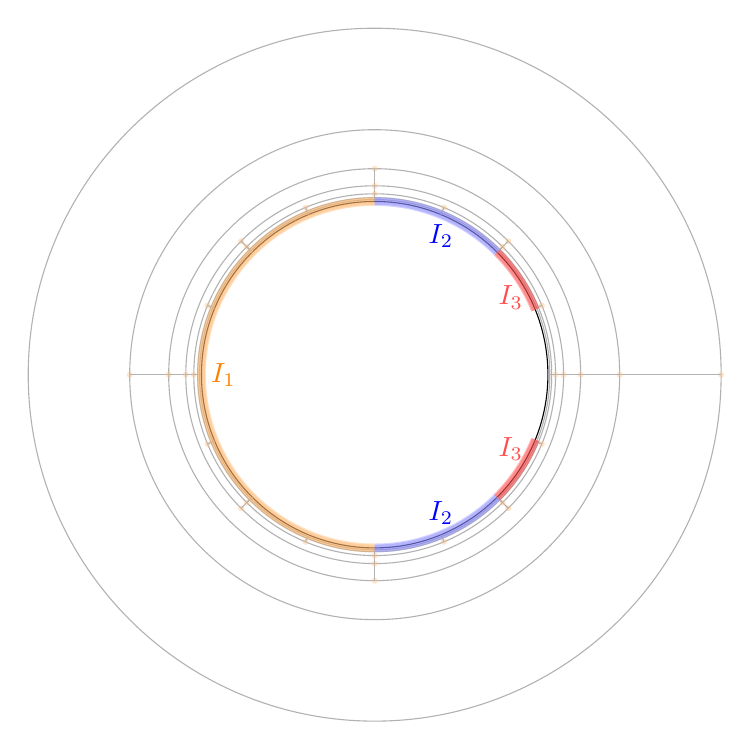
\begin{tikzpicture}[scale=2.2]

% The circles C_n
\draw (0,0) circle (1);
\foreach \i in {1,(1.0/2),(1.0/4),(1.0/8), (1.0/16), (1.0/32), (1.0/64)}{
\draw[black!30!white] (0,0) circle (2^\i);
}

% The central itinerary
% \draw [blue!70!white,-,
% 	double=blue!70!white,
% 	double distance=6\pgflinewidth, opacity=0.4,
% 	] 
%     (2,0) 
%  -- (2^0.5,0) 
%  arc (0:180:2^0.5) 
%  -- (-2^0.25,0) 
%  arc (180:90:2^0.25)
%  -- (0,2^0.0625)
%  arc (90:112.5:2^0.0625)
%  --(112.5:2^0.03125);


    
\foreach \j in {0,1,2,3,4}{
    \pgfmathsetmacro{\jtwo}{2.0^\j}
    \pgfmathsetmacro{\jthree}{(1.0/\jtwo)}
    \pgfmathsetmacro{\twopower}{2^\jthree}
    \foreach \angleone in {1,...,\jtwo}{
    \pgfmathsetmacro{\anglez}{360*\angleone}
    \fill[orange!50!white] (\anglez * \jthree: \twopower) circle (0.5pt)[opacity=0.4];
    \draw[black!30!white] (\anglez * \jthree: \twopower) -- (\anglez * \jthree: 1);	
    }
}

% \draw [blue!70!white,-,
	% double=blue!70!white,
	% double distance=4\pgflinewidth, opacity=0.4,
	% ] 


  		\draw [orange!60!white,-,
			double=orange!60!white,
			double distance=6\pgflinewidth, opacity=0.4,
			] (0,1) arc (90:270:1)
   node[midway, right,opacity=1, text=orange] {$I_1$};
		
		\draw [blue!40!white,-,
			double=blue!50!white,
			double distance=6\pgflinewidth, opacity=0.4,
			] (0,1) arc (90:45:1)
      node[midway, below,opacity=1, text=blue] {$I_2$};

		\draw [blue!40!white,-,
			double=blue!50!white,
			double distance=6\pgflinewidth, opacity=0.4,
			] (0,-1) arc (270:315:1)
   node[midway, above,opacity=1,text=blue] {$I_2$};

		\draw [red!70!white,-,
			double=red!70!white,
			double distance=6\pgflinewidth, opacity=0.4,
			] (45:1) arc (45:22:1)
   node[midway, below,opacity=1,xshift=-3, yshift=1] {$I_3$};

   
		\draw [red!   70!white,-,
			double=red!70!white,
			double distance=6\pgflinewidth, opacity=0.4,
			] (-45:1) arc (-45:-22:1)
   node[midway, above, xshift=-3,opacity=1] {$I_3$};

\end{tikzpicture}


 
\caption{First few parts of the departure decomposition $I_m$ of the circle.} 
\label{fig:departure-decomposition}

\end{figure}

		

